\documentclass[10pt,twocolumn]{article}
\usepackage[margin=0.75in]{geometry}                % See geometry.pdf to learn the layout options. There are lots.
\geometry{letterpaper}                   % ... or a4paper or a5paper or ... 
%\geometry{landscape}                % Activate for for rotated page geometry
%\usepackage[parfill]{parskip}    % Activate to begin paragraphs with an empty line rather than an indent
\setlength{\columnsep}{1cm}
\usepackage{graphicx}
\usepackage{amssymb}
\usepackage{epstopdf}
\usepackage{fullpage}
\usepackage[usenames]{color}
\usepackage{titlesec}
\usepackage{hyperref}
\usepackage{framed}
\usepackage{algorithmic}

\definecolor{light-gray}{gray}{0.45}
\definecolor{Blue}{rgb}{.2, 0,.5}
\newcommand{\solution}[1]{\textcolor{Blue}{\\{\bf Solution:} \\ #1}}  %Solution

\titleformat{\section}
{\color{black}\normalfont\Large\bfseries}
{\color{black}\thesection}{1em}{}

\titleformat{\subsection}
{\color{light-gray}\normalfont\large\bfseries}
{\color{light-gray}\thesubsection}{1em}{}

\DeclareGraphicsRule{.tif}{png}{.png}{`convert #1 `dirname #1`/`basename #1 .tif`.png}

\title{\Huge{\bf Algorithm 5: Ray}}
\author{Comp175: Introduction to Computer Graphics -- Spring 2014}
\date{Algorithm due:  {\bf Monday April 7th} at 11:59pm}                                         % Activate to display a given date or no date

\begin{document}
\maketitle
%\section{}
%\subsection{}

\begin{verbatim}
Your Names: Jayme Woogerd
            Louis Rassaby

Your CS Logins: jwoogerd
                lrassa01
\end{verbatim}

\section{Instructions}
Complete this assignment only with your teammate. When a numerical answer is required, provide a reduced fraction (i.e. 1/3) or at least three decimal places (i.e. 0.333). Show all work; write your answers on this sheet. This algorithm handout is worth 3\% of your final grade for the class.

\begin{framed}
\noindent{\bf[2 points]} The high-level view of our ray tracer is exactly the same as for intersect, except for a few additions. Below is the high-level pseudocode for {\tt Intersect}. What needs to be changed/added to make this a full-fledged raytracer? Just specify what changes need to be made {no pseudocode please.}

\footnotesize{
\begin{algorithmic}
\FOR{$point \in Canvas$}
	\STATE Cast a ray to find the nearest object
	\IF{ray intersects an object}
		\FOR{each light}
			\STATE Cast a ray to the light and evaluate the lighting equation\\
			\STATE $Canvas[pt] = Canvas[pt]+ color$ with only diffuse/ambient components\\
		\ENDFOR
	\ELSE 
		\STATE $Canvas[pt] =$ background color
	\ENDIF
\ENDFOR
\end{algorithmic}
\vspace{20mm}
\solution{
There are two modifications:
\begin{enumerate}
\item We need to check to see if the point is in shadow.
\item We need to modify the lighting equation to be the recursive lighting equation given on the assignment sheet.
\end{enumerate}
}
}

\vskip 5em
\end{framed}

\begin{framed}
\noindent{\bf[2 points]} Given a vector $\vec{v}$ and a surface normal $\vec{n}$, find the equation for the vector $\vec{r}$ which is the reflection of $\vec{v}$ about $\vec{n}$ (i.e. in the equal and opposite direction). Write your equation in terms of vector operations. How do you compute the color contributed by the reflected ray? Give a brief description.
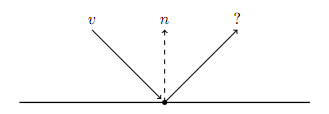
\includegraphics[width=2.8in]{reflection.png}
\solution{
We are solving for the reflected vector, $\vec{r}$.
\[ \vec{v_{||}} = (\vec{n} \cdot \vec{-v}) * \vec{n}\]
\[ \vec{v_{\perp}} = \vec{-v} - \vec{v_{||}} \]
\[ \vec{r} = \vec{v_{||}} + \vec{v_{\perp}} \]
Or...
\[ \vec{r} = 2\vec{n} * (\vec{n} \cdot (-\vec{v})) + \vec{v} \]
}
\end{framed}

\begin{framed}
\pagebreak
\noindent{\bf[1 point]} Is ray tracing a local or global illumination algorithm? Why?
\solution{
Ray tracing is a global illumination algorithm. In addition to an object's inherent lighting, ray tracing depends on other objects, ambient and diffuse light sources, and specular, reflective, and other lighting effects.
}
\end{framed}

\begin{framed}
\noindent{\bf[1 point]} For what two cases will an object (or portions of an object) not be affected by a light source? There are actually more than two cases, but we expect you to be able to list at least two; you can list more for extra credit.
\solution{
\begin{enumerate}
\item If it is occluded by (i.e. in the shadow of) another object relative to a light source.
\item If the light source is directly behind the object, relative to the eyepoint.
\item If an object has so much light in a channel that it is already fully lit and cannot be lit any more. This was particularly apparent during a4.
\item If a light source emits a light that cannot be absorbed by the object.
\end{enumerate}
}
\end{framed}

\begin{framed}
\noindent{\bf[2 points]} Recall that we can think of texture mapping in two steps. First, mapping from the object to the unit square, and second, mapping from the unit square to the texture map. Let $a$ and $b$ be the $x$ and $y$ values in the unit square that a particular point on an object gets mapped to in the first step. Note that $a$ and $b$ are calculated differently depending on the object. From here, how do you find the coordinates $(s, t)$ to look up in a texture map in terms of $a, b, u, v, w$ and $h$, where $u$ and $v$ are the number of repetitions in the $x$ and $y$ directions, respectively, $w$ is the texture width, and $h$ is the texture height?
\solution{
f
}
\end{framed}
\vskip 6em

\begin{framed}
\noindent{\bf[1 point]} How do you use the color from the texture map and the {\tt blend} value in the lighting equation?
\vskip 12em
\end{framed}

\begin{framed}
\noindent{\bf[1 point]}  What is the Phong lighting model used for? What is the purpose of its exponent?
\vskip 12em
\end{framed}

\section{How to Submit}

Hand in a PDF version of your solutions using the following command:
\begin{center}
 {\tt provide comp175 a5-alg}
 \end{center}
\end{document}  
